\documentclass[11pt,fleqn]{article} 
\usepackage[margin=0.8in, head=0.8in]{geometry} 
\usepackage{amsmath, amssymb, amsthm}
\usepackage{fancyhdr} 
\usepackage{palatino, url, multicol}
\usepackage{graphicx} 
\usepackage[all]{xy}
\usepackage{polynom} 
\usepackage{pdfsync}
\usepackage{enumerate}
\usepackage{framed}
\usepackage{setspace}
\usepackage{array,tikz}
\pagestyle{fancy} 
\lfoot{UAF Calculus 1}
\rfoot{review trig}

\begin{document}
\renewcommand{\headrulewidth}{0pt}
\newcommand{\blank}[1]{\rule{#1}{0.75pt}}
\renewcommand{\d}{\displaystyle}
\vspace*{-0.7in}
\begin{center}
  \large \sc{Worksheet: Review of Trigonometry}
\end{center}
\begin{enumerate}
\item \textbf{Unit Circle Definition}\\

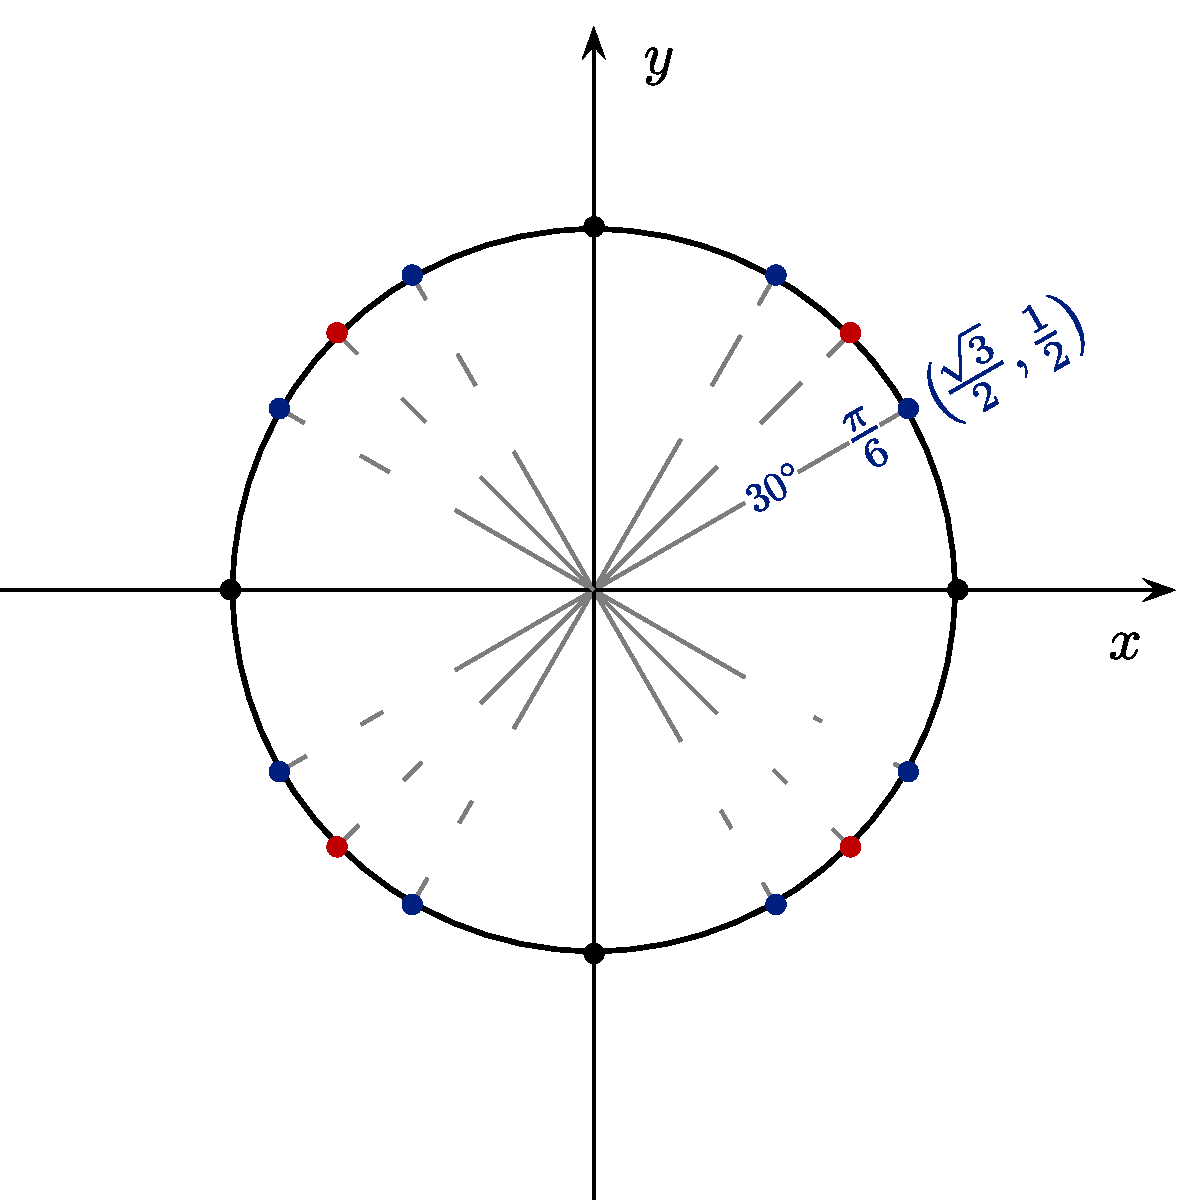
\includegraphics[scale=.6]{blank-unit-circle}

\vfill

(a) $\sin(4 \pi/3)=$ \hfill (b) $\cos(3\pi/4)=$ \hfill (c) $\tan(11\pi/6)=$ \hspace{.8in}\quad\\
\vfill
What is a radian?\\

\vfill

\newpage
\item \textbf{Right-triangle Definition}
\vfill
\item \textbf{Familiar Graphs} Use the previous work to construct and confirm the graphs of $f(\theta)=\sin(\theta)$, $f(\theta)=\cos(\theta)$, $f(\theta)=\tan(\theta)$.
\vspace{6in}
\newpage
\item Find \emph{all} solutions to the equations below. Show your reasoning.
\begin{multicols}{2}
\begin{enumerate}
\item $\cos x =1$
\vspace{.5in}
\item $\sin x =1$
\vspace{1in}
\columnbreak
\item $\tan x = 0$
\vspace{1in}
\item $\sin x = 1/2$ (Find all solutions in $[0,2\pi].$)
\vspace{.5in}
\end{enumerate}
\end{multicols}
\vfill
\item Convert $2\pi/3$ radians and $5\pi/7$ radians to degrees.
\vfill
\item Convert $20$ degrees to radians.
\vfill
\newpage
\item Without a calculator and without going back to the first pages (!!) evaluate:
  \begin{multicols}{3}{
      % make sure you added \usepackage{enumerate}
      \vspace*{-0.45in}
      \begin{enumerate}[(a)]
      \item $\sin (\frac{2 \pi}{3} )$
      \item $\cos( \frac{5 \pi}{4} )$
      \item $\tan(\frac{- \pi}4 )$
      \end{enumerate}}
  \end{multicols}
\vfill
\item A wooden ramp is to be built with one end on the ground and the other end at the top of a short staircase. If the top of the staircase is  4 ft from the ground and the angle between the ground and the ramp is to be $10^o$,  how long does the ramp need to be?\\
\vfill
\item Find $\cos \theta$ assuming that $\sin \theta = 2/7$ and $\theta$ is in the first quadrant.
\vspace{2in}
\end{enumerate}
\end{document}




\newpage
\item Find the equation of the line between the points $(-1,2)$ and $(3,6).$
\vfill
\item Assume $P(t)=\sqrt{4t+4}-2$ gives the distance traveled by a runner in the first 30 seconds of a race where  $t$ is measured in seconds and $P$ is measured in meters. (So the domain of $P$ is $[0,30].$)
\begin{enumerate}
\item Find the slope, $m$, of the line between the points $(3,P(3))$ and $(15,P(15)).$
\vfill
\item What should the units of $m$ be and why?
\vfill
\end{enumerate}
\end{enumerate}
\end{document}
%%%%%%%%%%%%
%%%%%%%%%%%%
%%%%%%%%%%%%
Functions can be
represented in a variety of ways. Specifically, there are four that we
will focus on during this course. They are:

\vskip1in


\textbf{Example 1:} (Graphically) Interpreting the graph of a function. The graph of
a function $f$ is shown below. Find the following:

\begin{quote}
  \begin{multicols}{2}{
      % make sure you added \usepackage{enumerate}
      \vspace*{-0.55in}
      \begin{enumerate}[a)]
      \item $f(1)$ and $f(5)$
      \item the domain of $f$
      \item the range of $f$
      \item For which value of $x$ is $f(x) = 4$?
      \item Where if $f$ increasing?
\columnbreak
\begin{center}
  \includegraphics[width=2.8in]{1-1-fig-6}
\end{center}
      \end{enumerate}}
\end{multicols}
\end{quote}
\vskip0.45in
\item Find the domain if each of the following:


\textbf{Example 2:} (Algebraically) If $f(x) = 3x^2 - x + 2$ find the
following. Are (b) and (c) different? 

\begin{quote}
  \begin{multicols}{2}{
      % make sure you added \usepackage{enumerate}
      \vspace*{-0.45in}
      \begin{enumerate}[(a)]
      \item $f(2)$
\vskip1in
      \item $f(a^2)$
\vskip1in
      \item $[f(a)]^2$
\columnbreak
      \item $\d \frac{f(a+h) - f(a)}{h}$
      \end{enumerate}}
  \end{multicols}
\end{quote}

\vskip2.5in


\textbf{Example 3:} Graph the following functions. Give the domain and
range. 
\begin{quote}
  \begin{multicols}{2}{
      % make sure you added \usepackage{enumerate}
      \vspace*{-0.45in}
      \begin{enumerate}[a)]
      \item $f(x) =
        \begin{cases}
          -1\; &\text{if} \; x \ge 2 \\
          7 - 2x \; & \text{if} \; x < 2
        \end{cases}$

        \begin{flushleft}
          \includegraphics[width=1.9in]{grid-print}
        \end{flushleft}

      \item $f(x) =
        \begin{cases}
          x+1 \; &\text{if} \; x \le - 1 \\
          x^2 \; &\text{if} \; x > -1
        \end{cases}$

           \begin{flushleft}
          \includegraphics[width=1.9in]{grid-print}
        \end{flushleft}
      \end{enumerate}}
  \end{multicols}
\end{quote}
\vskip0.5in
\textbf{Domain of a Function:} 

The \textbf{domain} of a function is the set of all possible values of
the input. One can find the domain of a function from a picture, but
it is also possible to do so from an equation. In many instances it is
easier to think about what operations are illegal and leave out the
numbers that break these operations. Remember, 

\begin{enumerate}
\item Thou shalt not divide by \blank{1in}. Set the \blank{1.5in}
  equal to zero. Leave these numbers out. 
\item Thou shalt not square root \blank{1in}. Set the stuff under the
  radical \blank{0.25in} zero and solve. Note, solving polynomial
  inqualities is not simple. 
\item Thou shalt not take the logaraithm of \blank{1in}. Set the stuff
  inside the logarithm \blank{0.25in} zero and solve. This process is
  quite similar to \# 2. 
\end{enumerate}


\textbf{Example 3:} Find the domain of each function. Give the domain
using interval notation. 
\begin{quote}
  \begin{multicols}{2}{
      % make sure you added \usepackage{enumerate}
      \vspace*{-0.45in}
      \begin{enumerate}[(a)]
      \item $f(x) = \d \frac{1}{x^4 - 16}$
      \item  $f(x) = \sqrt{x} + \sqrt{11 - x}$
      \end{enumerate}}
  \end{multicols}
\end{quote}
\vskip2in

\newpage
\textbf{Example 4:} Find the domain of each function. Give the domain
using interval notation. 
\begin{quote}
  \begin{multicols}{2}{
      % make sure you added \usepackage{enumerate}
      \vspace*{-0.45in}
      \begin{enumerate}[a)]
      \item $g(x) = \ln( x^2 - 4 )$
      \item $h(x) = \frac{1}{\sqrt{x^2 - 5x - 6}}$
      \end{enumerate}}
  \end{multicols}
\end{quote}


\vskip1.5in

\textbf{Example 6:} A rectangular storage container with an open top
has a volume of 10 $m^3$. The length of its base is twice the
width. Materials for the base cost \$10 per square meter and material
for the sides cost \$6 per square meter. Express the cost of materials
as a function of the width of the base.  Give the domain of the
function. 
\vskip2.5in

\subsection*{Symmetry}

\begin{itemize}
\item A function $f(x)$ is called even if \blank{1in}. An example is
  $f(x) = $ \blank{0.5in}. Even functions are symmetric about
  \blank{1in}.
\item A function $f(x)$ is called odd if \blank{1in}. An example is
  $f(x) = $ \blank{0.5in}. Odd functions are symmetric about the
  origin. 
\end{itemize}

\textbf{Example 7:} Determine whether the following functions are
even, odd, or neither. 


  \begin{multicols}{3}{
      % make sure you added \usepackage{enumerate}
      \vspace*{-0.45in}
      \begin{enumerate}[a)]
      \item $g(x) = e^x + 1$
      \item $f(x) = 1 + 3x^2 - x^4$
      \item $f(x) = \frac{x}{x^2+1}$
      \end{enumerate}}
  \end{multicols}




\end{document}